\section{Template similarity modelling}
\label{section:modelling-similarity}

Both the single-article retrieval setting and the page-aware scoring setting require comparing the internal topological structure of two templates $\templateobj{1}$ and $\templateobj{2}$, in order to assess how structurally similar or distinct their zonings are. In this context, standard metrics such as Intersection-over-Union (IoU) or Jaccard index (\secref{sec:sota-geometric-similarity}) are insufficient: they are sensitive to small misalignments, and in cases with no overlap they provide zero gradients, making optimization difficult~\cite{patil_layoutgmn_2021}. 

Two complementary similarity measures are proposed to address this:
\begin{itemize}
    \item \textbf{Template- and distance-based Intersection over Union}, an analytical, distance-IoU~\cite{zheng_distance-iou_2019} based measure that is fast to compute and requires no training data. Being analytical, however, it remains IoU-based, and therefore the misalignment issues described above can still persist.
    \item \textbf{Template-based Graph Matching Network}, a learned measure that captures richer topological relationships considering inner blocks and their classes. Because it requires training data, the former similarity measure is used to weakly label the triplets on which it is trained.
\end{itemize}
Both measures are presented in turn below, and are later compared empirically and qualitatively.

\subsection{Similarity measure 1: Template- and distance-based Intersection over Union ($\tdiou{\cdot}{\cdot}$)}

This first similarity measure is an analytical, geometry-based metric that provides a first approximation to layout similarity, without requiring any training data.

This similarity metric, coined Template- and distance-based Intersection over Union ($\tdiou{\cdot}{\cdot}$), which adapts the Distance-IoU loss~\cite{zheng_distance-iou_2019} to multi-element layouts, considers both the overlap between regions and the distance between their centers, providing a continuous measure of geometric alignment.

The computation of $\tdiou{\cdot}{\cdot}$ involves three steps: rescaling templates for fair comparison, matching elements of the same class, and summing the similarity of matched elements. Formally, for templates $\templateobj{1}$ and $\templateobj{2}$:
\begin{equation}
\tdiou{\templateobj{1}}{\templateobj{2}} = C_S \, C_M \, \frac{\sum_{(\zblock{1}{j},\zblockrescaled{2}{k}) \in M} \diouplusone{\zblock{1}{j}}{\zblockrescaled{2}{k}}}{|M|},
\label{eq:tdiou}
\end{equation}


where $\zblockrescaled{2}{k}$ are elements of $\tilde{\templateobj{2}}$, which corresponds to $\templateobj{2}$ rescaled to match $\templateobj{1}$ ($\Htemp{\tilde{\templateobj{2}}} = \Htemp{\templateobj{1}} $, $\Wtemp{\tilde{\templateobj{2}}} = \Wtemp{\templateobj{1}}$), $M$ is the set of matched element pairs, $C_S$ penalizes dimensional differences, and $C_M$ accounts for unmatched elements. The rest of this section gives more details about the different terms and notions introduced here.  

%TODO: Image about this

\subsubsection*{Similarity measure (\diouplusone{\templateobj{1}}{\templateobj{2}})}
\label{sec:tdiou:diouplusone}


Starting from a reimplementation using CGAL~\cite{cgal} of \diou{\templateobj{1}}{\templateobj{2}}~\cite{zheng_distance-iou_2019} in $[-1,1]$, \diouplusone{\templateobj{1}}{\templateobj{2}} is defined as:
\[
\diouplusone{\templateobj{1}}{\templateobj{2}} = \diou{\templateobj{1}}{\templateobj{2}} + 1,
\]
ensuring non-negative values. 

CGAL~\cite{cgal} was adopted for this reimplementation because template blocks may be arbitrary convex or concave polygons, possibly with holes, rather than simple axis-aligned rectangles. CGAL provides robust and fast C++ implementations of the polygon intersection and union operations this requires.
\subsubsection*{Rescaling and dimensional penalty}
\label{sec:tdiou:rescaling}

Templates are rescaled for element-wise comparison. Let $\tilde{\templateobj{2}}$ denote $\templateobj{2}$ rescaled to match $\templateobj{1}$. The penalty factor $C_S$ reduces similarity when $\templateobj{2}$ differs substantially from $\templateobj{1}$ in area, aspect ratio, or orientation:
\begin{align*} 
    C_S =& f_{\sigma_{1},\gamma_1}(\Htemp{\templateobj{1}}\Wtemp{\templateobj{1}} - \Htemp{\templateobj{2}}\Wtemp{\templateobj{2}}) \,
           f_{\sigma_2,\gamma_2}(\arctan(\Htemp{\templateobj{1}}/\Wtemp{\templateobj{1}}) - \arctan(\Htemp{\templateobj{2}}/\Wtemp{\templateobj{2}})) \nonumber\\
         & \, g_{\sigma_3,\gamma_3}((\arctan(\Htemp{\templateobj{1}}/\Wtemp{\templateobj{1}}) - \pi/4)(\arctan(\Htemp{\templateobj{2}}/\Wtemp{\templateobj{2}}) - \pi/4)),
\end{align*}
with
\[
f_{\sigma,\gamma}(t) = \exp\left(-\frac{(t/\gamma)^2}{2\sigma^2}\right), \quad
g_{\sigma,\gamma}(t) =
\begin{cases}
\exp\left(\frac{t/\gamma}{\sigma}\right), & t < 0,\\
1, & t \ge 0.
\end{cases}
\]

Each of the three factors composing $C_S$ targets a distinct source of dimensional mismatch:
\begin{itemize}
    \item the first factor, $f_{\sigma_1,\gamma_1}$, penalizes differences in total area between $\templateobj{1}$ and $\templateobj{2}$;
    \item the second factor, $f_{\sigma_2,\gamma_2}$, penalizes differences in aspect ratio between the two templates;
    \item the third factor, $g_{\sigma_3,\gamma_3}$, further penalizes the case where $\templateobj{1}$ and $\templateobj{2}$ fall on opposite sides of a square aspect ratio (e.g., one portrait-oriented and the other landscape-oriented), since such an orientation flip is perceptually more disruptive than a comparable difference in aspect ratio alone.
\end{itemize}
Both $f_{\sigma,\gamma}$ and $g_{\sigma,\gamma}$ decay smoothly toward zero as their argument grows in magnitude, so $C_S$ approaches zero, and the overall similarity \tdiou{\templateobj{1}}{\templateobj{2}} collapses accordingly, increasing the difference between $\templateobj{1}$ and $\templateobj{2}$.

\subsubsection*{Element matching and penalty}
\label{sec:tdiou:matching}
Elements $\zblock{1}{j} \in \templateobj{1}$ and $\zblockrescaled{2}{k} \in \tilde{\templateobj{2}}$ are matched based on $\diouplusone{\templateobj{1}}{\templateobj{2}}$ similarity and class correspondence, formulated as an assignment problem solvable with the Hungarian algorithm~\cite{hungarian}. The set of matched pairs is $M$. Unmatched elements are penalized via:
\[
C_M = \frac{1}{2 \, \Htemp{\templateobj{1}}\Wtemp{\templateobj{1}}} \sum_{(\zblock{1}{j},\zblockrescaled{2}{k}) \in M} \big( area(\zblock{1}{j} + area(\zblockrescaled{2}{k}) \big).
\]
This ensures \tdiou{\templateobj{1}}{\templateobj{2}} accounts for both matched element quality and structural differences.
%TODO figure for matching

\subsection{Similarity measure 2: Template-based Graph Matching Network ($\gmn{\cdot}{\cdot}$)}

This second similarity measure is a learned measure that captures richer topological relationships considering inner blocks and their classes, as a way to prevent the misalignment issues of IoU-based measures.

The proposed method is a Graph Matching Network (GMN) architecture~\cite{patil_layoutgmn_2021}, here referred to as \gmnNetwork, was implemented and retrained for the purpose of this work, following the cross-graph attention mechanism and triplet-based training scheme described in \secref{sec:sota-gmn}. Templates are represented as directed, fully connected graphs over their constituent elements, in the same manner as LayoutGMN, and \gmnNetwork is trained on triplets built from $\tdiou{\cdot}{\cdot}$ thresholds rather than plain Intersection-over-Union. Consequently, \gmnNetwork produces a similarity function, denoted $\gmn{\cdot}{\cdot}$, that can be applied to any pair of templates $\templateobj{1}$ and $\templateobj{2}$. Following the sign convention of the LayoutGMN implementation, this raw score is negative by construction and satisfies $\gmn{\templateobj{1}}{\templateobj{2}} = 0$ if the templates are identical, growing more negative as their structures diverge.

The use of the $\gmn{\cdot}{\cdot}$ metric varies depending on the application; in single-article context (\secref{section:template-retrieval-single-article}), the absolute value of this metric is used to define the distance for clustering and retrieval. In the page-aware setting of \neuralmethod\ (\secref{sec:gwes-gmn-mapping}), the same score is instead mapped into a bounded $[0,1]$ affinity through a Gaussian kernel, since that context requires a normalized similarity matrix rather than an unbounded distance.


\subsection{Empirical comparison}

\subsubsection*{Motivation}

To assess which similarity measure better reflects human perception, an online study was conducted. Each trial consisted of: (1) a reference template $\templateobj{R}$ shown for 2 seconds, followed by (2) a selection scene where participants chose the template most similar to $\templateobj{R}$ between two options $\templateobj{O_1}$ and $\templateobj{O_2}$. This design specifically targets immediate perceptual judgment rather than deliberate analysis, since participants are given only a few seconds to decide.

\subsubsection*{Research questions and hypothesis}

This study tests whether $\tdiou{\cdot}{\cdot}$ or $\gmn{\cdot}{\cdot}$ better aligns with immediate human judgments of layout similarity.

\subsubsection*{Experimental design}

\paragraph{Clustering using both methods}

Using the distance $d(\cdot,\cdot)$ defined by:
\begin{equation}
d_{tdIoU}(\templateobj{1},\templateobj{2}) = |\tdiou{\templateobj{1}}{\templateobj{2}}|,
\label{eq:clustering-distance-definition}
\end{equation}
templates are organized via agglomerative clustering with a threshold $\tdiouclusterthreshold$. Starting from singleton clusters, pairs of clusters are merged when their average inter-template distance is below $\tdiouclusterthreshold$. This produces a set of clusters $\tdiouclusters$.

At the same time, a set of clusters $\gmnclusters$ can be generated using an analog distance $d_{GMN}(\templateobj{1},\templateobj{2}) = |\gmn{\templateobj{1}}{\templateobj{2}}|$, and the corresponding inter-template maximum average distance of $\gmnclusterthreshold$.

Note that both $\tdiouclusterthreshold$ and $\gmnclusterthreshold$ were set to produce a reasonable, but also equivalent and comparable number of clusters between the methods. Specifically, $\tdiouclusterthreshold = 1.1$ and $\gmnclusterthreshold=2.8$, producing $|\tdiouclusters| = 80$ and $|\gmnclusters| = 81$ respectively, with a similar distribution.

\paragraph{Triplet definition}
Each trial involved a triplet $(R,O_1,O_2)$. $\templateobj{O_1}$ was chosen as a neighbor of $\templateobj{R}$ according to \tdiou{\templateobj{R}}{\templateobj{O_1}} but not \gmn{\templateobj{R}}{\templateobj{O_1}}, and $O_2$ as a neighbor according to \gmn{\templateobj{R}}{\templateobj{O_2}} but not \tdiou{\templateobj{R}}{\templateobj{O_2}}.  40 randomnly-selected triplets were generated this rule (examples in \figref{fig:online_experiment}(b)).

\paragraph{Experimental protocol}
Participants completed a short questionnaire on reading habits, followed by four blocks of 40 trials each, and a post-experiment questionnaire on their experience. Responses were collected via \emph{Labvanced}~\cite{labvanced}, yielding $42 \times 4$ votes per triplet.

\subsubsection*{Population}

The study recruited $42$ anonymous participants via \emph{Prolific}~\cite{prolific}.

\subsubsection*{Results}
Across all trials and participants, votes were evenly split between $O_1$ and $O_2$, resulting in a global 50:50 ratio between both methods. This indicates that neither similarity measure dominates when results are aggregated.

However, a finer-grained analysis at the triplet level reveals a more structured pattern. \figref{fig:online_experiment}(a) shows the percentage of $O_2$ (GMN) selections for each triplet, along with the interquartile range defined by Q1 and Q3 (25\%--75\% of responses). Only six triplets ($15\%$) fall (in average) within the 40\%--60\% range, indicating near-indifference between the two measures. In contrast, most triplets exhibit a clear preference, as reflected by asymmetric interquartile ranges.

Focusing on the interquartile interval, $45\%$ of the triplets (triplets $\{23,\dots,40\}$) show a majority preference for $\gmn{\cdot}{\cdot}$, while $40\%$ of the triplets (triplets $\{1,\dots,15\}$) favor $\tdiou{\cdot}{\cdot}$. This suggests that participant judgments are highly dependent on the specific structural and geometric characteristics of the templates involved.

To better understand these differences, two representative triplets (10 and 35) are illustrated in \figref{fig:online_experiment}(b). In triplet 10, participants predominantly selected $O_1$, consistent with the high geometric overlap captured by $\tdiou{\cdot}{\cdot}$, despite differences in the presence of small layout elements. Conversely, in triplet 35, participants favored $O_2$, where $\gmn{\cdot}{\cdot}$ captures higher structural similarity, while $\tdiou{\cdot}{\cdot}$ is more strongly influenced by variations in the size of dominant elements such as the main image and body text.


\begin{figure}[thbp]
    \centering
    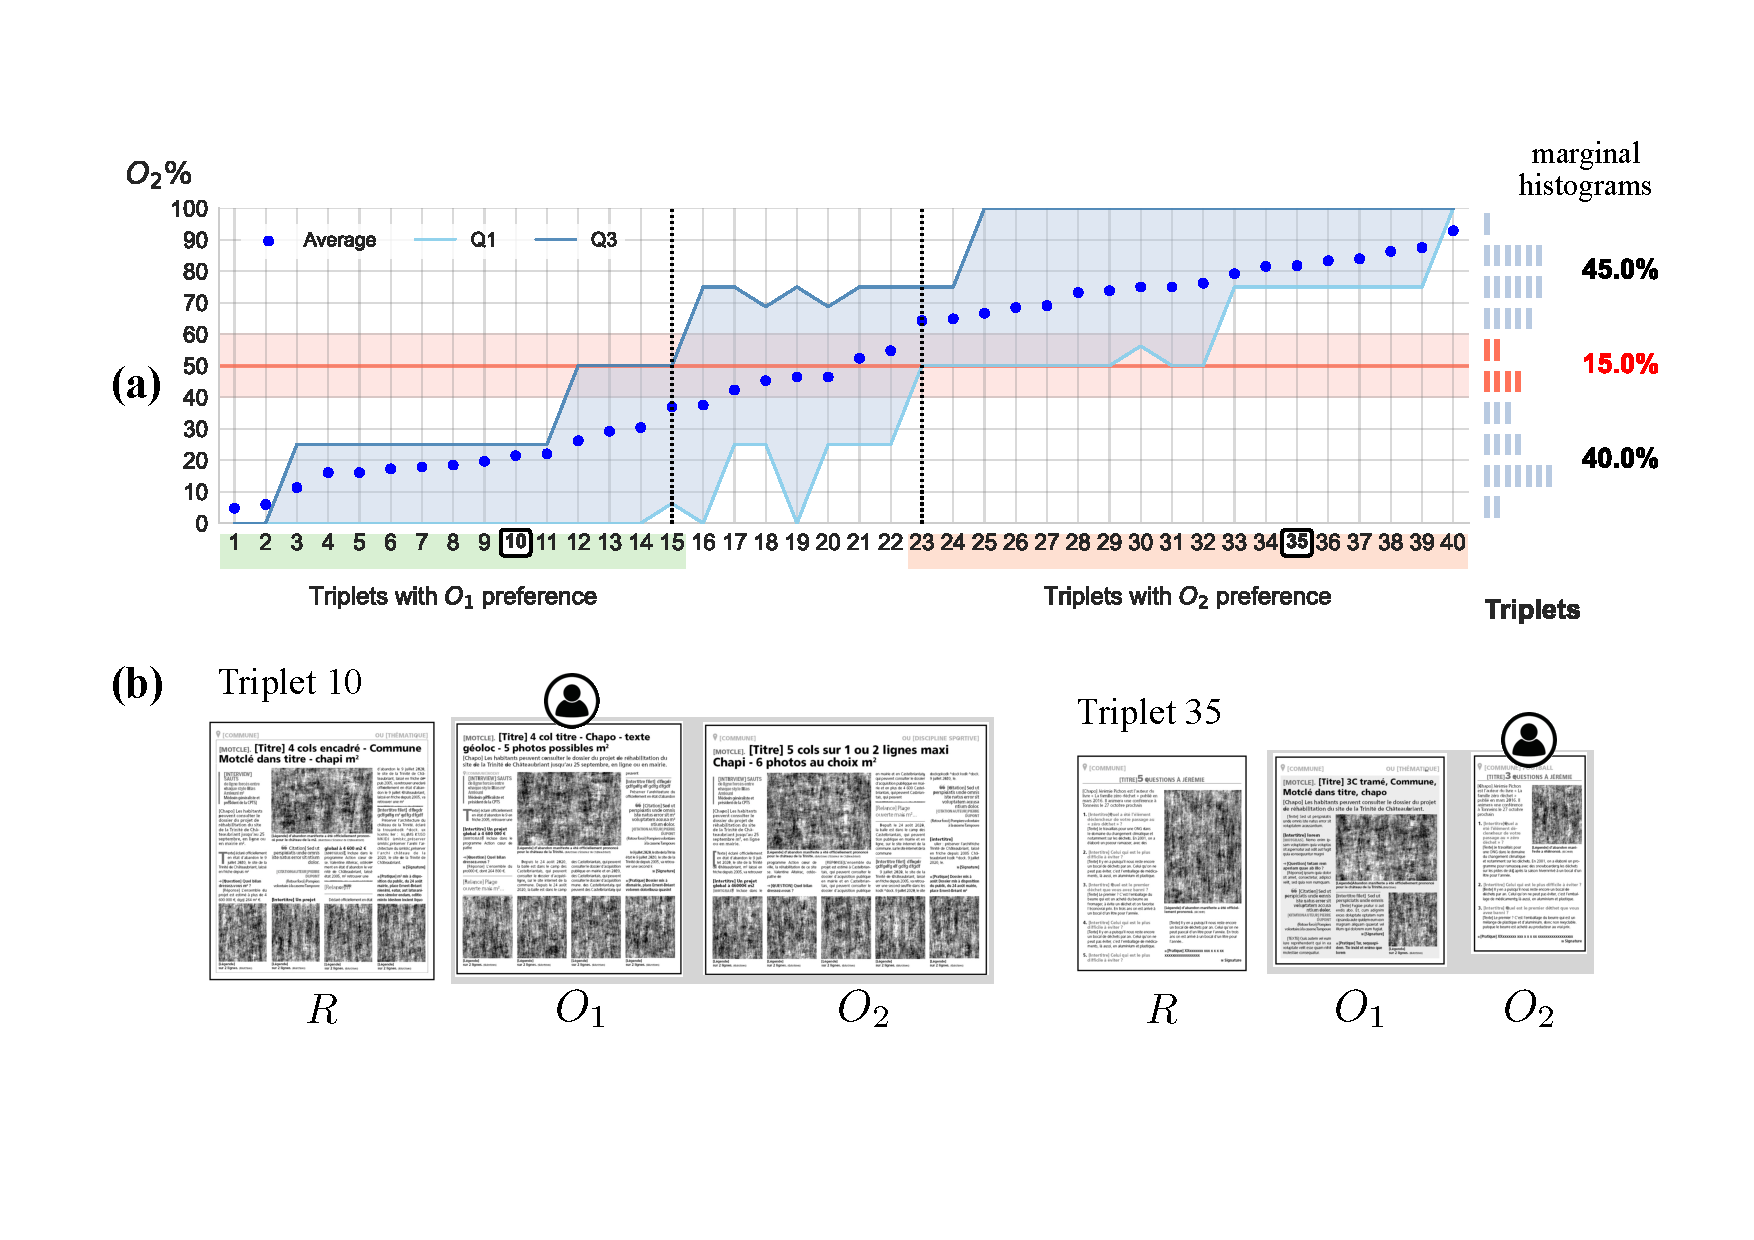
\includegraphics[width=\widthForOneImage]{img/online_experiment.pdf}
    \caption{\label{fig:online_experiment} 
Results of the online experiment.
(a) Percentage of $O_2$  selections for each of the 40 triplets. Each point represents the average percentage of $O_2$ selections, with the shaded area indicating the interquartile range ($Q1$–$Q3$). Two groups are highlighted: triplets \{1,\dots,15\} (green), where participants mainly selected $O_1$ ($\tdiou{\cdot}{\cdot}$), and triplets \{23,\dots,40\} (orange), where participants mainly selected $O_2$ ($\gmn{\cdot}{\cdot}$). A central band ($40\%$–$60\%$) where no clear preference was established. The marginal histogram (right) counts the frequency of triplets in $10\%$ intervals, where each block represents a single triplet. The bold percentage labels indicate the total proportion of the triplets falling into each of the three categories.
(b) Example triplets from each group. Individual participant choices are represented by a human-shaped icon.
    }
\end{figure}

\subsection{Qualitative comparison}
%todo complete this


This analysis lead to the selection of $\gmn{\cdot}{\cdot}$ as the main similarity measure to be used in this work.
%TODO maybe extend unless the previous section is conclusive enough